\section{Рабочий проект}

\subsection{Классы, используемые при разработке сайта}

Программная система состоит из сущностей, выраженных классами и структурами языка C++. Их взаимодействие реализуется через встроенные механизмы наследования и представлено в диаграмме UML (рис. \ref{uml:image}).

\afterpage{
  \begin{landscape}
    \begin{figure}[p]
      \centering
      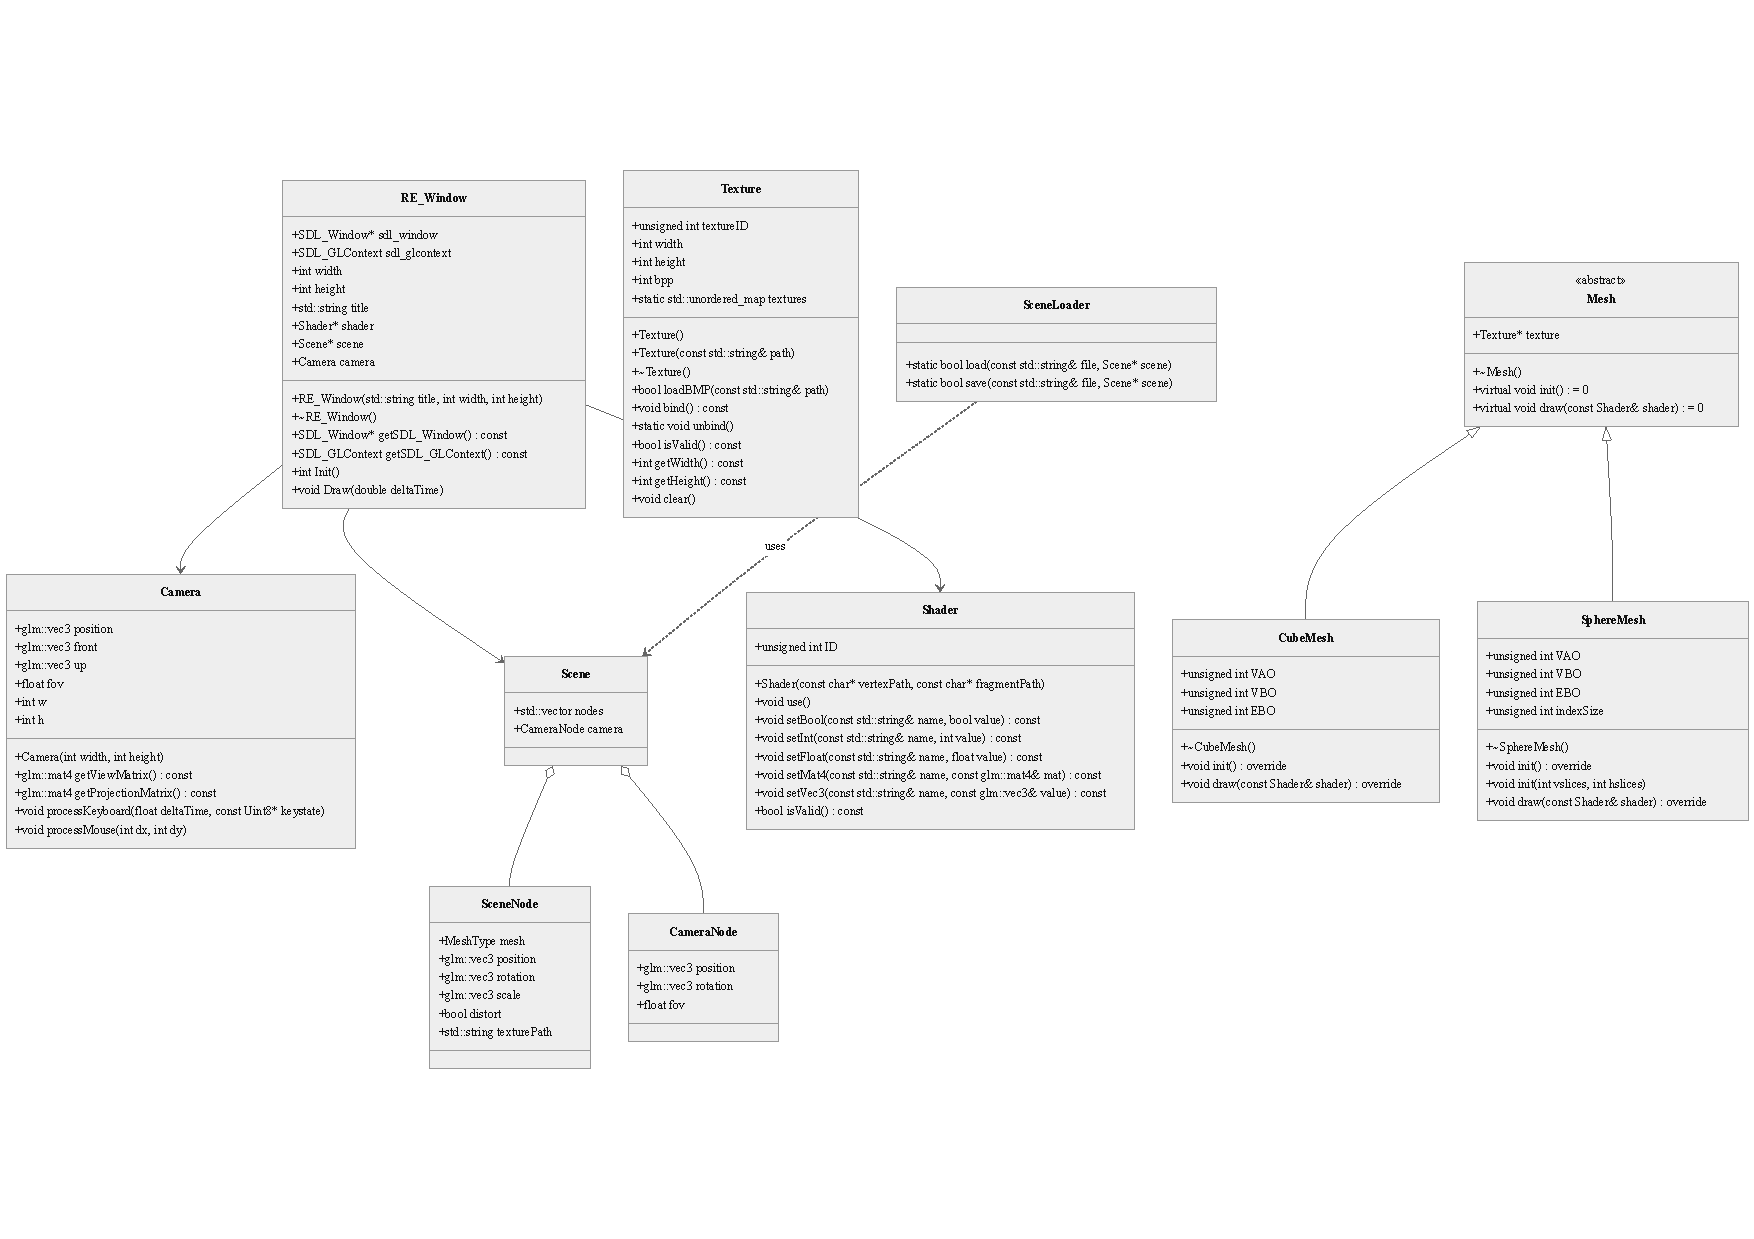
\includegraphics[width=1.6\textwidth]{uml.pdf}
      \caption{Диаграмма UML}
      \label{uml:image}
    \end{figure}
  \end{landscape}
}

\subsubsection{Класс Renderer}
Класс Renderer отвечает за управление процессом отрисовки трёхмерной сцены. Он инкапсулирует логику взаимодействия с графическим API (OpenGL), управляет объектами сцены, шейдерами и камерой. Класс не занимается напрямую созданием окна или обработкой событий, предполагая, что эти задачи решаются внешними компонентами.

Спецификация класса Renderer представлена в таблице \ref{tab:renderer_spec}.

\begin{xltabular}{\textwidth}{|X|l|X|}
    \caption{Спецификация класса Renderer\label{tab:renderer_spec}}\\ \hline
    \centrow Поле/Метод & \centrow Тип & \centrow Описание \\ \hline
    \endfirsthead
    \continuecaption{Продолжение таблицы \ref{tab:renderer_spec}}
    \centrow Поле/Метод & \centrow Тип & \centrow Описание \\ \hline 
    \finishhead

    \multicolumn{3}{|l|}{Приватные поля} \\ \hline
    width & int & Ширина области рендеринга в пикселях. \\ \hline
    height & int & Высота области рендеринга в пикселях. \\ \hline
    scene & Scene* & Указатель на объект сцены, содержащий все объекты для отображения. \\ \hline
    \multicolumn{3}{|l|}{Методы} \\ \hline
    Renderer(int width, int height) & конструктор & Конструктор класса. Инициализирует размеры области рендеринга. \\ \hline
    getScene() & Scene* & Возвращает указатель на текущую сцену. \\ \hline
    setScene(Scene* scene) & void & Устанавливает активную сцену для рендеринга. \\ \hline
    setShader(const char* vertexPath, const char* fragmentPath) & void & Загружает и устанавливает шейдерную программу по путям к вершинному и фрагментному шейдерам. \\ \hline
    getWidth() & int & Возвращает ширину области рендеринга. \\ \hline
    getHeight() & int & Возвращает высоту области рендеринга. \\ \hline
    draw(unsigned long ticks) & void & Выполняет отрисовку одного кадра. ticks -- текущее время в миллисекундах. \\ \hline
\end{xltabular}

Вспомогательная функция \texttt{initRenderer(int width, int height)} (определена в пространстве имен REngine, заголовочный файл \texttt{Renderer.h}) создает и возвращает указатель на новый экземпляр класса \texttt{Renderer}, инициализированный с заданной шириной и высотой.

\subsubsection{Управление окном и главный цикл}
Функциональность, связанная с созданием окна приложения, управлением главным циклом и закрытием окна, сосредоточена в пространстве имен \texttt{REngine} (см. заголовочный файл \texttt{Engine.h}). Этот модуль предоставляет набор функций и перечисление для кодов ошибок.

\paragraph{Перечисление WindowError}
Перечисление \texttt{WindowError} определяет константы для кодов ошибок, которые могут возникнуть при операциях с окном.

Спецификация перечисления WindowError представлена в таблице \ref{tab:windowerror_spec}.

\begin{xltabular}{\textwidth}{|l|X|}
    \caption{Спецификация перечисления WindowError\label{tab:windowerror_spec}}\\ \hline
    \centrow Значение & \centrow Описание \\ \hline
    \endfirsthead
    \continuecaption{Продолжение таблицы \ref{tab:windowerror_spec}}
    \centrow Значение & \centrow Описание \\ \hline 
    \finishhead
    WINDOW\_ALREADY\_EXISTS & Окно уже было создано. \\ \hline
    WINDOW\_CREATE\_FAILED & Не удалось создать окно SDL. \\ \hline
    GL\_CONTEXT\_CREATE\_FAILED & Не удалось создать контекст OpenGL. \\ \hline
    RENDERER\_INIT\_FAILED & Не удалось инициализировать рендерер. \\ \hline
\end{xltabular}

\paragraph{Функции управления окном}
Набор функций для управления жизненным циклом окна и приложения.

Спецификация функций управления окном представлена в таблице \ref{tab:windowfuncs_spec}.

\begin{xltabular}{\textwidth}{|X|l|X|}
    \caption{Спецификация функций управления окном\label{tab:windowfuncs_spec}}\\ \hline
    \centrow Функция & \centrow Возвращаемый тип & \centrow Описание \\ \hline
    \endfirsthead
    \continuecaption{Продолжение таблицы \ref{tab:windowfuncs_spec}}
    \centrow Функция & \centrow Возвращаемый тип & \centrow Описание \\ \hline 
    \finishhead
    createWindow(const char* title, int width = 0, int height = 0) & int & Инициализирует SDL, создает окно приложения и контекст OpenGL. \texttt{title} - заголовок окна. \texttt{width} и \texttt{height} - размеры окна; если 0, используется полноэкранный режим. Возвращает 0 при успехе или код ошибки из \texttt{WindowError} при неудаче. \\ \hline
    mainLoop() & void & Запускает главный цикл приложения. В цикле обрабатываются события ввода, обновляется состояние сцены и происходит отрисовка. Цикл продолжается до тех пор, пока не будет получен сигнал о закрытии окна. \\ \hline
    setScene(REngine::Scene* scene) & void & Устанавливает текущую сцену для рендеринга. \\ \hline
    getScene() & REngine::Scene* & Возвращает указатель на текущую сцену. \\ \hline
    setShader(const char* vertexPath, const char* fragmentPath) & void & Устанавливает шейдерную программу для рендеринга. \\ \hline
    destroyWindow() & void & Удаляет окно SDL, контекст OpenGL и освобождает ресурсы SDL. Должна вызываться перед завершением работы приложения. \\ \hline
\end{xltabular}

\subsubsection{Структура SceneNode}
Структура \texttt{SceneNode} представляет собой отдельный объект (узел) в трехмерной сцене. Она содержит информацию о геометрии объекта, его трансформациях (позиция, поворот, масштаб), материале и текстурах.

Спецификация структуры SceneNode представлена в таблице \ref{tab:scenenode_spec}.

\begin{xltabular}{\textwidth}{|l|l|X|}
    \caption{Спецификация структуры SceneNode\label{tab:scenenode_spec}}\\ \hline
    \centrow Поле & \centrow Тип & \centrow Описание \\ \hline
    \endfirsthead
    \continuecaption{Продолжение таблицы \ref{tab:scenenode_spec}}
    \centrow Поле & \centrow Тип & \centrow Описание \\ \hline 
    \finishhead
    mesh & Mesh* & Указатель на объект геометрии (меш). \\ \hline
    position & glm::vec3 & Позиция объекта в мировых координатах. Значение по умолчанию: (0,0,0). \\ \hline
    rotation & glm::vec3 & Углы поворота объекта вокруг осей X, Y, Z в градусах. Значение по умолчанию: (0,0,0). \\ \hline
    scale & glm::vec3 & Масштаб объекта по осям X, Y, Z. Значение по умолчанию: (1,1,1). \\ \hline
    shininess & float & Коэффициент блеска материала объекта. Используется в модели освещения Фонга. Значение по умолчанию: 32.0. \\ \hline
    distort & bool & Флаг, указывающий, нужно ли применять эффект искажения к текстуре объекта. Значение по умолчанию: false. \\ \hline
    texturePath & std::string & Путь к файлу основной текстуры объекта (diffuse map). \\ \hline
    specularPath & std::string & Путь к файлу текстуры для карты отражений (specular map). \\ \hline
\end{xltabular}

\subsubsection{Структура DirLight}
Структура \texttt{DirLight} описывает параметры направленного источника света в сцене.

Спецификация структуры DirLight представлена в таблице \ref{tab:dirlight_spec}.

\begin{xltabular}{\textwidth}{|l|l|X|}
    \caption{Спецификация структуры DirLight\label{tab:dirlight_spec}}\\ \hline
    \centrow Поле & \centrow Тип & \centrow Описание \\ \hline
    \endfirsthead
    \continuecaption{Продолжение таблицы \ref{tab:dirlight_spec}}
    \centrow Поле & \centrow Тип & \centrow Описание \\ \hline 
    \finishhead
    direction & glm::vec3 & Вектор направления света. \\ \hline
    ambient & glm::vec3 & Интенсивность окружающего света. Компоненты (R,G,B) в диапазоне [0,1]. \\ \hline
    diffuse & glm::vec3 & Интенсивность диффузного света. Компоненты (R,G,B) в диапазоне [0,1]. \\ \hline
    specular & glm::vec3 & Интенсивность зеркального света. Компоненты (R,G,B) в диапазоне [0,1]. \\ \hline
\end{xltabular}

\subsubsection{Структура PointLight}
Структура \texttt{PointLight} описывает параметры точечного источника света. Точечный свет излучается из одной точки во всех направлениях, и его интенсивность убывает с расстоянием.

Спецификация структуры PointLight представлена в таблице \ref{tab:pointlight_spec}.

\begin{xltabular}{\textwidth}{|l|l|X|}
    \caption{Спецификация структуры PointLight\label{tab:pointlight_spec}}\\ \hline
    \centrow Поле & \centrow Тип & \centrow Описание \\ \hline
    \endfirsthead
    \continuecaption{Продолжение таблицы \ref{tab:pointlight_spec}}
    \centrow Поле & \centrow Тип & \centrow Описание \\ \hline 
    \finishhead
    position & glm::vec3 & Позиция источника света в мировых координатах. \\ \hline
    constant & float & Константный коэффициент затухания интенсивности света. \\ \hline
    linear & float & Линейный коэффициент затухания интенсивности света. \\ \hline
    quadratic & float & Квадратичный коэффициент затухания интенсивности света. \\ \hline
    ambient & glm::vec3 & Цвет окружающего света. \\ \hline
    diffuse & glm::vec3 & Цвет диффузного света. \\ \hline
    specular & glm::vec3 & Цвет зеркального света. \\ \hline
\end{xltabular}

\subsubsection{Класс Camera}
Класс Camera отвечает за управление виртуальной камерой в трехмерном пространстве. Он предоставляет методы для установки и получения позиции и ориентации камеры, вычисления матриц вида и проекции, а также для относительного перемещения и вращения. Камера использует библиотеку GLM для математических операций.

Спецификация класса Camera представлена в таблице \ref{tab:camera_spec}.

\begin{xltabular}{\textwidth}{|X|l|X|}
    \caption{Спецификация класса Camera\label{tab:camera_spec}}\\ \hline
    \centrow Поле/Метод & \centrow Тип & \centrow Описание \\ \hline
    \endfirsthead
    \continuecaption{Продолжение таблицы \ref{tab:camera_spec}}
    \centrow Поле/Метод & \centrow Тип & \centrow Описание \\ \hline 
    \finishhead

    \multicolumn{3}{|l|}{Поля} \\ \hline
    position & glm::vec3 & Позиция камеры в мировых координатах. \\ \hline
    fov & float & Угол обзора (поле зрения) камеры в градусах. \\ \hline
    w & int & Ширина окна отрисовки, используется для расчета матрицы проекции. \\ \hline
    h & int & Высота окна отрисовки, используется для расчета матрицы проекции. \\ \hline
    front & glm::vec3 & (Приватное) Вектор, указывающий направление камеры. \\ \hline
    up & glm::vec3 & (Приватное) Вектор, указывающий "верх" для камеры. \\ \hline
    \multicolumn{3}{|l|}{Методы} \\ \hline
    Camera() & конструктор & Конструктор по умолчанию. \\ \hline
    Camera(int width, int height) & конструктор & Конструктор. Инициализирует камеру с указанной шириной и высотой окна. \\ \hline
    setRotation(float rx, float ry, float rz) & void & Устанавливает углы поворота камеры по осям X, Y, Z (в градусах). \\ \hline
    getRotation() const & glm::vec3 & Возвращает текущие углы поворота камеры по осям X, Y, Z (в градусах) в виде вектора. \\ \hline
    getViewMatrix() const & glm::mat4 & Вычисляет и возвращает матрицу вида (view matrix). \\ \hline
    getProjectionMatrix() const & glm::mat4 & Вычисляет и возвращает матрицу проекции (projection matrix). \\ \hline
    moveRelative(float dx, float dy, float dz) & void & Перемещает камеру относительно ее текущей ориентации на заданные смещения. \\ \hline
    rotateRelative(float drx, float dry, float drz) & void & Поворачивает камеру относительно ее текущей ориентации на заданные углы (в градусах). \\ \hline
\end{xltabular}

\subsubsection{Структура Scene}
Структура \texttt{Scene} является контейнером для всех элементов, составляющих трехмерную сцену. Она объединяет информацию об объектах, камере, источниках света и других параметрах окружения.

Спецификация структуры Scene представлена в таблице \ref{tab:scene_spec}.

\begin{xltabular}{\textwidth}{|l|l|X|}
    \caption{Спецификация структуры Scene\label{tab:scene_spec}}\\ \hline
    \centrow Поле & \centrow Тип & \centrow Описание \\ \hline
    \endfirsthead
    \continuecaption{Продолжение таблицы \ref{tab:scene_spec}}
    \centrow Поле & \centrow Тип & \centrow Описание \\ \hline 
    \finishhead
    nodes & std::vector<SceneNode> & Список всех объектов (узлов) в сцене. \\ \hline
    camera & Camera & Конфигурация камеры сцены. \\ \hline
    skyColor & glm::vec3 & Цвет неба (фона) сцены. Компоненты (R,G,B) в диапазоне [0,1]. Значение по умолчанию: (0.63, 0.63, 0.85). \\ \hline
    dirLight & DirLight & Параметры направленного источника света в сцене. \\ \hline
    pointLights & std::vector<PointLight> & Список точечных источников света в сцене. \\ \hline
\end{xltabular}

\subsubsection{Перечисление MeshType}
Перечисление \texttt{MeshType} определяет типы геометрических примитивов, которые могут быть использованы в сцене:

\begin{itemize}
    \item \texttt{Cube} -- кубический примитив;
    \item \texttt{Sphere} -- сферический примитив;
    \item \texttt{Custom} -- пользовательский примитив.
\end{itemize}

\subsubsection{Класс Mesh}
Класс \texttt{Mesh} представляет собой геометрию для отрисовки в сцене. Он инкапсулирует данные о вершинах, индексах, а также управляет буферами OpenGL (VAO, VBO, EBO) для эффективной отрисовки. Класс также может содержать указатели на текстуры.

Спецификация класса Mesh представлена в таблице \ref{tab:mesh_spec}.

\begin{xltabular}{\textwidth}{|X|l|X|}
    \caption{Спецификация класса Mesh\label{tab:mesh_spec}}\\ \hline
    \centrow Поле/Метод & \centrow Тип & \centrow Описание \\ \hline
    \endfirsthead
    \continuecaption{Продолжение таблицы \ref{tab:mesh_spec}}
    \centrow Поле/Метод & \centrow Тип & \centrow Описание \\ \hline 
    \finishhead
    \multicolumn{3}{|l|}{Публичные поля} \\ \hline
    texture & Texture* & Указатель на основную текстуру объекта (diffuse). \\ \hline
    specularTexture & Texture* & Указатель на текстуру отражений (specular map). \\ \hline
    \multicolumn{3}{|l|}{Приватные поля} \\ \hline
    vertices & std::vector<float> & Вектор вершин меша. \\ \hline
    VAO & unsigned int & Идентификатор Vertex Array Object. \\ \hline
    VBO & unsigned int & Идентификатор Vertex Buffer Object. \\ \hline
    EBO & unsigned int & Идентификатор Element Buffer Object. \\ \hline
    indexSize & unsigned int & Количество индексов для отрисовки. \\ \hline
    min & glm::vec3 & Минимальные координаты AABB (bounding box). \\ \hline
    max & glm::vec3 & Максимальные координаты AABB. \\ \hline
    \multicolumn{3}{|l|}{Методы} \\ \hline
    Mesh(std::vector<float> vertices, std::vector<unsigned> indices) & конструктор & Конструктор. Инициализирует меш с заданными вершинами и индексами. \\ \hline
    \textasciitilde Mesh() & деструктор & Деструктор. Освобождает ресурсы OpenGL. \\ \hline
    draw(const Shader \& shader) & void & Отрисовывает меш с использованием указанного шейдера. \\ \hline
    computeAABB() & void & Вычисляет Axis-Aligned Bounding Box (AABB) для меша на основе его вершин. \\ \hline
    getMin() & const glm::vec3\& & Возвращает минимальные координаты AABB. \\ \hline
    getMax() & const glm::vec3\& & Возвращает максимальные координаты AABB. \\ \hline
    \multicolumn{3}{|l|}{Статические методы} \\ \hline
    createCube() & static Mesh & Создает и возвращает меш стандартного куба. \\ \hline
    createSphere(int vslices = 100, int hslices = 100) & static Mesh & Создает и возвращает меш сферы с указанным числом вертикальных (vslices) и горизонтальных (hslices) сегментов. \\ \hline
\end{xltabular}

\subsubsection{Класс Shader}
Класс \texttt{Shader} инкапсулирует логику загрузки, компиляции, связывания и использования шейдерных программ в OpenGL. Он позволяет загружать вершинные и фрагментные шейдеры из файлов или использовать встроенные по умолчанию, а также предоставляет удобные методы для установки uniform-переменных различных типов.

Спецификация класса Shader представлена в таблице \ref{tab:shader_spec}.

\begin{xltabular}{\textwidth}{|X|l|X|}
    \caption{Спецификация класса Shader\label{tab:shader_spec}}\\ \hline
    \centrow Поле/Метод & \centrow Тип & \centrow Описание \\ \hline
    \endfirsthead
    \continuecaption{Продолжение таблицы \ref{tab:shader_spec}}
    \centrow Поле/Метод & \centrow Тип & \centrow Описание \\ \hline 
    \finishhead
    \multicolumn{3}{|l|}{Публичные поля} \\ \hline
    ID & unsigned int & Идентификатор скомпилированной и связанной шейдерной программы OpenGL. \\ \hline
    \multicolumn{3}{|l|}{Публичные методы} \\ \hline
    Shader(const char* vertexPath = NULL, const char* fragmentPath = NULL) & конструктор & Конструктор класса. Загружает, компилирует и связывает вершинный и фрагментный шейдеры. \texttt{vertexPath} - путь к файлу вершинного шейдера, \texttt{fragmentPath} - путь к файлу фрагментного шейдера. Если пути не указаны (NULL), используются встроенные шейдеры по умолчанию. \\ \hline
    use() & void & Активирует данную шейдерную программу для использования в текущем контексте рендеринга OpenGL. \\ \hline
    setBool(const std::string \&name, bool value) const & void & Устанавливает значение uniform-переменной типа boolean в шейдере. \texttt{name} - имя переменной, \texttt{value} - значение. \\ \hline
    setInt(const std::string \&name, int value) const & void & Устанавливает значение uniform-переменной типа int в шейдере. \texttt{name} - имя переменной, \texttt{value} - значение. \\ \hline
    setFloat(const std::string \&name, float value) const & void & Устанавливает значение uniform-переменной типа float в шейдере. \texttt{name} - имя переменной, \texttt{value} - значение. \\ \hline
    setMat4(const std::string \&name, const glm::mat4 \&mat) const & void & Устанавливает значение uniform-переменной типа mat4 (матрица 4x4) в шейдере. \texttt{name} - имя переменной, \texttt{mat} - матрица. \\ \hline
    setVec3(const std::string \&name, const glm::vec3 \&value) const & void & Устанавливает значение uniform-переменной типа vec3 (вектор из 3-х компонентов) в шейдере. \texttt{name} - имя переменной, \texttt{value} - вектор. \\ \hline
    isValid() const & bool & Проверяет, была ли шейдерная программа успешно скомпилирована и связана. Возвращает \texttt{true}, если \texttt{ID != 0}, иначе \texttt{false}. \\ \hline
    \multicolumn{3}{|l|}{Приватные методы} \\ \hline
    checkCompileErrors(unsigned int shader, std::string type) & void & Вспомогательный метод для проверки ошибок компиляции или связывания шейдеров. \texttt{shader} - идентификатор объекта шейдера или программы, \texttt{type} - строка, указывающая тип проверяемого объекта ("VERTEX", "FRAGMENT" или "PROGRAM"). \\ \hline
\end{xltabular}

\subsubsection{Класс Texture}
Класс Texture предназначен для загрузки, хранения и управления текстурными данными, которые используются для наложения изображений на поверхности 3D-объектов. В текущей реализации поддерживается загрузка текстур из файлов формата BMP. Класс инкапсулирует взаимодействие с OpenGL для создания и управления текстурными объектами, а также предоставляет статический кеш для загруженных текстур, чтобы избежать повторной загрузки одних и тех же файлов.

Спецификация класса Texture представлена в таблице \ref{tab:texture_spec}.

\begin{xltabular}{\textwidth}{|X|X|X|}
    \caption{Спецификация класса Texture\label{tab:texture_spec}}\\ \hline
    \centrow Поле/Метод & \centrow Тип & \centrow Описание \\ \hline
    \endfirsthead
    \continuecaption{Продолжение таблицы \ref{tab:texture_spec}}
    \centrow Поле/Метод & \centrow Тип & \centrow Описание \\ \hline 
    \finishhead
    \multicolumn{3}{|l|}{Приватные поля} \\ \hline
    textureID & unsigned int & Идентификатор текстурного объекта OpenGL. Используется для привязки и управления текстурой в графическом конвейере. \\ \hline
    width & int & Ширина загруженной текстуры в пикселях. \\ \hline
    height & int & Высота загруженной текстуры в пикселях. \\ \hline
    bpp & int & Количество битов на пиксель в загруженной текстуре. \\ \hline
    \multicolumn{3}{|l|}{Статические публичные поля} \\ \hline
    textures & static std::unordered\_map <std::string, Texture*> & Статический ассоциативный массив (кеш) для хранения загруженных текстур. Ключом является путь к файлу текстуры. \\ \hline
    \multicolumn{3}{|l|}{Публичные методы} \\ \hline
    Texture() & конструктор & Конструктор по умолчанию. \\ \hline
    Texture(const std::string\& path) & конструктор & Конструктор, загружающий текстуру из указанного файла BMP с помощью метода \texttt{loadBMP}. \\ \hline
    \textasciitilde Texture() & деструктор & Деструктор класса. Освобождает ресурсы, связанные с текстурным объектом OpenGL, вызывая \texttt{clear()}. \\ \hline
    loadBMP(const std::string\& path) & bool & Загружает текстуру из файла формата BMP. Читает заголовки BMP, извлекает данные пикселей и вызывает \texttt{loadToGL} для загрузки в OpenGL. Возвращает \texttt{true} при успешной загрузке, иначе \texttt{false}. \\ \hline
    genFromColor(float r, float g, float b) & bool & Генерирует простую одноцветную текстуру размером 1x1 пиксель. \texttt{r, g, b} - компоненты цвета в диапазоне [0.0, 1.0]. Вызывает \texttt{loadToGL}. Возвращает \texttt{true} при успехе. \\ \hline
    bind() const & void & Привязывает текстуру (делает ее активной на текстурном юните 0) для использования в последующих операциях рендеринга. \\ \hline
    isValid() const & bool & Проверяет, была ли текстура успешно загружена и инициализирована (\texttt{textureID != 0}). \\ \hline
    getWidth() const & int & Возвращает ширину текстуры в пикселях. \\ \hline
    getHeight() const & int & Возвращает высоту текстуры в пикселях. \\ \hline
    \multicolumn{3}{|l|}{Статические публичные методы} \\ \hline
    unbind() & static void & Отвязывает текущую активную текстуру от текстурного юнита 0. \\ \hline
    \multicolumn{3}{|l|}{Приватные методы} \\ \hline
    loadToGL(std::vector <unsigned char>\& rgbData, int minFilter, int magFilter) & void & Загружает данные пикселей \texttt{rgbData} в объект текстуры OpenGL. Устанавливает параметры фильтрации (\texttt{minFilter}, \texttt{magFilter}) и режим повторения. \\ \hline
    clear() & void & Освобождает ресурсы текстурного объекта OpenGL, если он был создан (\texttt{textureID != 0}). \\ \hline
\end{xltabular}

\subsubsection{Класс InputHandler}
Класс InputHandler представляет собой статический класс, отвечающий за обработку пользовательского ввода от клавиатуры и мыши. Он использует библиотеку SDL2 для получения событий и предоставляет интерфейс для регистрации callback-функций на различные события ввода, такие как нажатие, отпускание и удержание клавиш, движение мыши, нажатие кнопок мыши и прокрутка колесика. Класс также хранит текущее состояние клавиш и позицию мыши.

Спецификация класса InputHandler представлена в таблице \ref{tab:inputhandler_spec}.

\begin{xltabular}{\textwidth}{|X|X|X|}
    \caption{Спецификация класса InputHandler\label{tab:inputhandler_spec}}\\ \hline
    \centrow Поле/Метод & \centrow Тип & \centrow Описание \\ \hline
    \endfirsthead
    \continuecaption{Продолжение таблицы \ref{tab:inputhandler_spec}}
    \centrow Поле/Метод & \centrow Тип & \centrow Описание \\ \hline 
    \finishhead

    \multicolumn{3}{|l|}{Типы данных (using)} \\ \hline
    KeyCallback & std::function<void()> & Тип для callback-функции при нажатии/отпускании клавиши. \\ \hline
    HoldKeyCallback & std::function<void(float)> & Тип для callback-функции при удержании клавиши (аргумент - deltaTime). \\ \hline
    MouseMotionCallback & std::function<void(int, int, int, int)> & Тип для callback-функции при движении мыши (x, y, xrel, yrel). \\ \hline
    MouseButtonCallback & std::function<void(int, int, int)> & Тип для callback-функции при нажатии/отпускании кнопки мыши (x, y, button). \\ \hline
    MouseWheelCallback & std::function<void(int, int)> & Тип для callback-функции при прокрутке колесика мыши (x, y смещения). \\ \hline
    \multicolumn{3}{|l|}{Статические поля (приватные)} \\ \hline
    keyStates\_ & std::unordered \_map<SDL\_Keycode, bool> & Хранит текущее состояние клавиш (нажата/отпущена). \\ \hline
    keyDownCallbacks\_ & std::unordered \_map<SDL\_Keycode, KeyCallback> & Карта callback-функций для события нажатия клавиши. \\ \hline
    keyUpCallbacks\_ & std::unordered \_map<SDL\_Keycode, KeyCallback> & Карта callback-функций для события отпускания клавиши. \\ \hline
    keyHoldCallbacks\_ & std::unordered \_map<SDL\_Keycode, HoldKeyCallback> & Карта callback-функций для события удержания клавиши. \\ \hline
    mouseButtonDown\-Callbacks\_ & std::unordered \_map<Uint8, MouseButtonCallback> & Карта callback-функций для события нажатия кнопки мыши. \\ \hline
    mouseButtonUp\-Callbacks\_ & std::unordered \_map<Uint8, MouseButtonCallback> & Карта callback-функций для события отпускания кнопки мыши. \\ \hline
    mouseMotionCallback\_ & MouseMotionCallback & Callback-функция для события движения мыши. \\ \hline
    mouseWheelCallback\_ & MouseWheelCallback & Callback-функция для события прокрутки колесика мыши. \\ \hline
    mousePosition\_ & glm::vec2 & Текущая позиция курсора мыши. \\ \hline
    mouseRelativeMotion\_ & glm::vec2 & Относительное смещение мыши с последнего кадра. \\ \hline
    \multicolumn{3}{|l|}{Статические методы} \\ \hline
    init() & static void & Инициализирует обработчик ввода. \\ \hline
    handleEvent(const SDL\_Event\& event) & static bool & Обрабатывает входящее событие SDL. Возвращает true, если событие было обработано. \\ \hline
    update(float deltaTime) & static void & Обновляет состояние ввода, вызывает callback-функции для удерживаемых клавиш. deltaTime - время с прошлого кадра. \\ \hline
    setKeyDownCallback (SDL\_Keycode key, KeyCallback callback) & static void & Устанавливает callback-функцию для события нажатия указанной клавиши. \\ \hline
    setKeyUpCallback (SDL\_Keycode key, KeyCallback callback) & static void & Устанавливает callback-функцию для события отпускания указанной клавиши. \\ \hline
    setKeyHoldCallback (SDL\_Keycode key, HoldKeyCallback callback) & static void & Устанавливает callback-функцию для события удержания указанной клавиши. \\ \hline
    setMouseMotionCallback (MouseMotionCallback callback) & static void & Устанавливает callback-функцию для события движения мыши. \\ \hline
    setMouseButtonDown\-Callback (Uint8 button, MouseButtonCallback callback) & static void & Устанавливает callback-функцию для события нажатия указанной кнопки мыши. \\ \hline
    setMouseButtonUp\-Callback (Uint8 button, MouseButtonCallback callback) & static void & Устанавливает callback-функцию для события отпускания указанной кнопки мыши. \\ \hline
    setMouseWheelCallback (MouseWheelCallback callback) & static void & Устанавливает callback-функцию для события прокрутки колесика мыши. \\ \hline
    isKeyDown (SDL\_Keycode key) & static bool & Проверяет, нажата ли указанная клавиша в данный момент. \\ \hline
    getMousePosition() & static glm::vec2 & Возвращает текущую позицию курсора мыши. \\ \hline
    getMouseRelativeMotion () & static glm::vec2 & Возвращает относительное смещение мыши с последнего кадра. \\ \hline
\end{xltabular}

\subsubsection{Структура Plane}
Структура \texttt{Plane} представляет собой математическую плоскость в трехмерном пространстве, определяемую нормалью и расстоянием от начала координат. Используется для определения границ области видимости камеры (\texttt{Frustum}).

Спецификация структуры Plane представлена в таблице \ref{tab:plane_spec}.

\begin{xltabular}{\textwidth}{|X|l|X|}
    \caption{Спецификация структуры Plane\label{tab:plane_spec}}\\ \hline
    \centrow Поле/Метод & \centrow Тип & \centrow Описание \\ \hline
    \endfirsthead
    \continuecaption{Продолжение таблицы \ref{tab:plane_spec}}
    \centrow Поле/Метод & \centrow Тип & \centrow Описание \\ \hline 
    \finishhead
    \multicolumn{3}{|l|}{Поля} \\ \hline
    normal & glm::vec3 & Нормаль плоскости. Значение по умолчанию: (0.0f, 1.0f, 0.0f). \\ \hline
    distance & float & Расстояние от начала координат до плоскости вдоль ее нормали. Значение по умолчанию: 0.0f. \\ \hline
    \multicolumn{3}{|l|}{Методы} \\ \hline
    setNormalAndDistance(const glm::mat4\& projView, uint8\_t axis, bool positive) & void & Устанавливает нормаль и расстояние плоскости на основе матрицы проекции-вида, оси и направления. \\ \hline
\end{xltabular}

\subsubsection{Структура Frustum}
Структура \texttt{Frustum} определяет усеченную пирамиду видимости камеры. Она состоит из шести плоскостей (\texttt{Plane}), которые ограничивают видимое пространство. Используется для эффективного отсечения объектов, находящихся вне поля зрения камеры (frustum culling).

Спецификация структуры Frustum представлена в таблице \ref{tab:frustum_spec}.

\begin{xltabular}{\textwidth}{|X|l|X|}
    \caption{Спецификация структуры Frustum\label{tab:frustum_spec}}\\ \hline
    \centrow Поле/Метод & \centrow Тип & \centrow Описание \\ \hline
    \endfirsthead
    \continuecaption{Продолжение таблицы \ref{tab:frustum_spec}}
    \centrow Поле/Метод & \centrow Тип & \centrow Описание \\ \hline 
    \finishhead
    \multicolumn{3}{|l|}{Конструкторы} \\ \hline
    Frustum(const Camera\& camera, float aspect) & конструктор & Конструктор. Инициализирует шесть плоскостей усеченной пирамиды видимости на основе параметров камеры и соотношения сторон. \\ \hline
    \multicolumn{3}{|l|}{Поля} \\ \hline
    top & Plane & Верхняя плоскость отсечения. \\ \hline
    bottom & Plane & Нижняя плоскость отсечения. \\ \hline
    left & Plane & Левая плоскость отсечения. \\ \hline
    right & Plane & Правая плоскость отсечения. \\ \hline
    near & Plane & Ближняя плоскость отсечения. \\ \hline
    far & Plane & Дальняя плоскость отсечения. \\ \hline
    \multicolumn{3}{|l|}{Методы} \\ \hline
    isBoxInFrustum(const glm::vec3\& min, const glm::vec3\& max) const & bool & Проверяет, пересекается ли или полностью содержится ли ограничивающий параллелепипед (AABB), заданный минимальными и максимальными координатами, внутри усеченной пирамиды видимости. \\ \hline
\end{xltabular}


\subsection{Модульное тестирование}

Для обеспечения качества и надёжности работы информационной системы был разработан комплекс модульных тестов. Тесты включают в себя проверку корректности работы всех компонентов системы, а также тестирование различных сценариев использования.

Для разработки тестов был использован фреймворк Google Test. Он обеспечивает множество необходимых методов для написания модульных тестов, удобную интеграцию со средой разработки и системой сборки CMake.

% В попытках достичь максимальной эффективности тестирования, в процессе написания тестов был использован модуль gcovr. Он позволяет оценить степень покрытия кода тестами и выявить ветви и строки, которые не затронуты тестами. По результатам анализа были созданы HTML-отчёты, визуально отображающие качество покрытия кода тестами.

% Также, для выявления неоптимизированных участков кода был использован инструмент gprof, идущий в комплекте с MinGW. Он позволяет оценить время выполнения функций и выявить участки, которые необходимо заменить более оптимальными алгоритмами.

Модульный тест для класса Camera представлен на рисунке \ref{unitCamera:image}, для класса Renderer -- на рисунке \ref{unitRenderer:image}, для класса Shader -- на рисунке \ref{unitShader:image}, для класса Scene -- на рисунке \ref{unitScene:image}, для функции mainLoop -- на рисунке \ref{unitMainLoop:image}, для функции mainLoop -- на рисунке \ref{unitMainLoop:image}.

\begin{figure}[ht]
\begin{lstlisting}[language=C++]
TEST(Camera, DefaultViewProjection) {
    const int w = 800, h = 600;
    REngine::Camera cam(w, h);

    glm::mat4 view = cam.getViewMatrix();

    glm::mat4 proj = cam.getProjectionMatrix();

    EXPECT_NE(glm::determinant(view), 0.0f);
    EXPECT_NE(glm::determinant(proj), 0.0f);

    glm::vec3 initialPos = cam.position;
    cam.moveRelative(1.0f, 0.0f, 0.0f);
    EXPECT_NE(glm::length(cam.position - initialPos), 0.0f);

    glm::vec3 initialRotation = cam.getRotation();
    cam.rotateRelative(10.0f, 10.0f, 10.0f);
    glm::vec3 newRotation = cam.getRotation();
    EXPECT_NE(initialRotation.x, newRotation.x);
}
\end{lstlisting}  
\caption{Модульный тест класса Camera}
\label{unitCamera:image}
\end{figure}

\begin{figure}[ht]
\begin{lstlisting}[language=C++]
TEST(Renderer, Initialization) {
    if (SDL_Init(SDL_INIT_VIDEO) < 0) {
        FAIL() << "SDL could not initialize! SDL_Error: " << SDL_GetError();
    }
    SDL_Window* window = SDL_CreateWindow("Test", 
        SDL_WINDOWPOS_UNDEFINED, SDL_WINDOWPOS_UNDEFINED, 
        800, 600, 
        SDL_WINDOW_OPENGL | SDL_WINDOW_HIDDEN);
    ASSERT_NE(window, nullptr) << "Window could not be created!";

    SDL_GLContext context = SDL_GL_CreateContext(window);
    ASSERT_NE(context, nullptr) << "OpenGL context could not be created!";

    REngine::Renderer* renderer = REngine::initRenderer(800, 600);
    ASSERT_NE(renderer, nullptr) << "Renderer initialization failed";

    REngine::Scene scene;
    renderer->setScene(&scene);

    renderer->setShader(NULL, NULL);

    REngine::Scene* scenePtr = renderer->getScene();
    EXPECT_NE(scenePtr, nullptr);
    
    EXPECT_EQ(renderer->getWidth(), 800);
    EXPECT_EQ(renderer->getHeight(), 600);

    delete renderer;
    SDL_GL_DeleteContext(context);
    SDL_DestroyWindow(window);
    SDL_Quit();
}
\end{lstlisting}  
\caption{Модульный тест класса Renderer}
\label{unitRenderer:image}
\end{figure}

\begin{figure}[ht]
\begin{lstlisting}[language=C++]
TEST(Shader, Compilation) {
    const std::string vert_shader =
        "#version 330 core\n"
        "layout(location = 0) in vec3 aPos;\n"
        "void main() {\n"
        "    gl_Position = vec4(aPos, 1.0);\n"
        "}\n";

    const std::string frag_shader =
        "#version 330 core\n"
        "out vec4 FragColor;\n"
        "void main() {\n"
        "    FragColor = vec4(1.0, 0.0, 0.0, 1.0);\n"
        "}\n";

    std::string vert_path = "test_vert.glsl";
    std::string frag_path = "test_frag.glsl";
    std::ofstream vert_file(vert_path);
    std::ofstream frag_file(frag_path);
    vert_file << vert_shader;
    frag_file << frag_shader;
    vert_file.close();
    frag_file.close();

    if (SDL_Init(SDL_INIT_VIDEO) < 0) {
        FAIL() << "SDL could not initialize! SDL_Error: " << SDL_GetError();
    }

    SDL_Window* window = SDL_CreateWindow("Test", SDL_WINDOWPOS_UNDEFINED,
                                            SDL_WINDOWPOS_UNDEFINED, 640, 480, SDL_WINDOW_OPENGL);
    SDL_GLContext context = SDL_GL_CreateContext(window);

    REngine::Shader* shader = new REngine::Shader(vert_path.c_str(), frag_path.c_str());
    ASSERT_TRUE(shader->isValid()) << "Shader compilation failed";

    delete shader;
    SDL_GL_DeleteContext(context);
    SDL_DestroyWindow(window);
    std::remove(vert_path.c_str());
    std::remove(frag_path.c_str());
    SDL_Quit();
}
\end{lstlisting}  
\caption{Модульный тест класса Shader}
\label{unitShader:image}
\end{figure}

\begin{figure}[ht]
\begin{lstlisting}[language=C++]
TEST(Scene, NodeManipulation) {
    REngine::Scene scene;
    scene.camera = REngine::Camera(640, 480);
    
    REngine::SceneNode node1;
    node1.position = glm::vec3(1, 2, 3);
    node1.rotation = glm::vec3(45, 0, 0);
    node1.scale = glm::vec3(2);
    node1.shininess = 64.0f;
    node1.distort = true;
    node1.texturePath = "test_texture.bmp";
    
    scene.nodes.push_back(node1);
    ASSERT_EQ(scene.nodes.size(), 1);
    
    EXPECT_EQ(scene.nodes[0].position, glm::vec3(1, 2, 3));
    EXPECT_EQ(scene.nodes[0].rotation, glm::vec3(45, 0, 0));
    EXPECT_EQ(scene.nodes[0].scale, glm::vec3(2));
    EXPECT_FLOAT_EQ(scene.nodes[0].shininess, 64.0f);
    EXPECT_TRUE(scene.nodes[0].distort);
    EXPECT_EQ(scene.nodes[0].texturePath, "test_texture.bmp");
    
    scene.camera.position = glm::vec3(0, 0, 5);
    EXPECT_EQ(scene.camera.position, glm::vec3(0, 0, 5));

    scene.camera.setRotation(45.0f, 30.0f, 0.0f);
    glm::vec3 rotation = scene.camera.getRotation();
    EXPECT_FLOAT_EQ(rotation.x, 45.0f);
    EXPECT_FLOAT_EQ(rotation.y, 30.0f);

    glm::mat4 view = scene.camera.getViewMatrix();
    glm::mat4 proj = scene.camera.getProjectionMatrix();
    EXPECT_NE(glm::determinant(view), 0.0f);
    EXPECT_NE(glm::determinant(proj), 0.0f);

    scene.dirLight.direction = glm::vec3(-0.2f, -1.0f, -0.3f);
    scene.dirLight.ambient = glm::vec3(0.2f);
    scene.dirLight.diffuse = glm::vec3(0.5f);
    scene.dirLight.specular = glm::vec3(1.0f);
    
    EXPECT_EQ(scene.dirLight.direction, glm::vec3(-0.2f, -1.0f, -0.3f));
    EXPECT_EQ(scene.dirLight.ambient, glm::vec3(0.2f));
    EXPECT_EQ(scene.dirLight.diffuse, glm::vec3(0.5f));
    EXPECT_EQ(scene.dirLight.specular, glm::vec3(1.0f));
}
\end{lstlisting}  
\caption{Модульный тест класса Scene}
\label{unitScene:image}
\end{figure}

\begin{figure}[ht]
\begin{lstlisting}[language=C++]
TEST(Engine, WindowCreation) {
    REngine::Scene scene;
    
    REngine::SceneNode n_sphere, n_noTexture, n_texture, n_specular, n_alpha, n_garbage, n_garbageWithBm, n_16bit, n_notReal;
    n_texture.texturePath = "uv-test.bmp";
    n_specular.specularPath = "uv-test.bmp";
    n_alpha.texturePath = "alpha.bmp";
    n_garbage.texturePath = "garbage.bmp";
    n_garbageWithBm.texturePath = "garbage_with_bm.bmp";
    n_16bit.texturePath = "16bit.bmp";
    n_notReal.texturePath = "not_real.bmp";

    std::vector<REngine::SceneNode> nodes = {n_noTexture, n_texture, n_specular, n_alpha, n_garbage, n_garbageWithBm, n_16bit, n_notReal};

    for (auto& node : nodes) {
        node.mesh = new REngine::Mesh(REngine::Mesh::createCube());
        node.mesh->computeAABB();
        scene.nodes.push_back(node);
    }
    n_sphere.mesh = new REngine::Mesh(REngine::Mesh::createSphere());
    n_sphere.mesh->computeAABB();
    scene.nodes.push_back(n_sphere);

    scene.dirLight.direction = glm::vec3(-1, -1, -1);
    scene.dirLight.ambient = glm::vec3(0.2f);
    scene.dirLight.diffuse = glm::vec3(0.5f);
    scene.dirLight.specular = glm::vec3(1.0f);

    scene.camera = REngine::Camera(800, 600);
    scene.camera.position = glm::vec3(0, 0, 5);
    scene.camera.setRotation(0.0f, -90.0f, 0.0f);

    REngine::createWindow("test", 800, 600);
    REngine::setScene(&scene);

    REngine::setShader(NULL, NULL);

    REngine::mainLoop();

    REngine::destroyWindow();
}
\end{lstlisting}  
\caption{Модульный тест функции mainLoop}
\label{unitMainLoop:image}
\end{figure}
\clearpage

\subsection{Системное тестирование}

На рисунке \ref{scene:image} представлен пример загруженной сцены, визуализированной движком.
% \newpage % при необходимости можно переносить рисунок на новую страницу
\begin{figure}[H] % H - рисунок обязательно здесь, или переносится, оставляя пустоту
\center{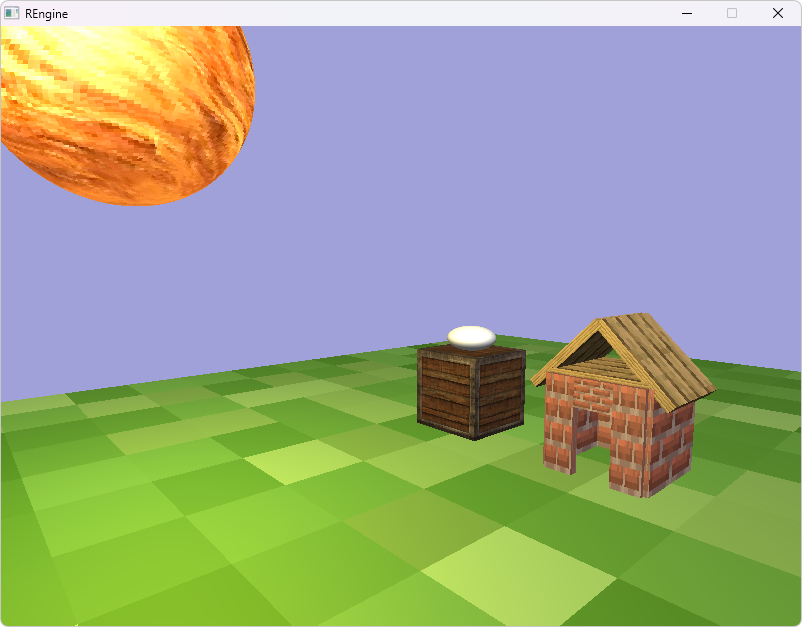
\includegraphics[width=1\linewidth]{scene.png}}
\caption{Загруженная сцена}
\label{scene:image}
\end{figure}

На рисунке \ref{culling:image} представлена сцена, тестирующая функционал отсечения невидимых поверхностей.

\begin{figure}[ht]
\center{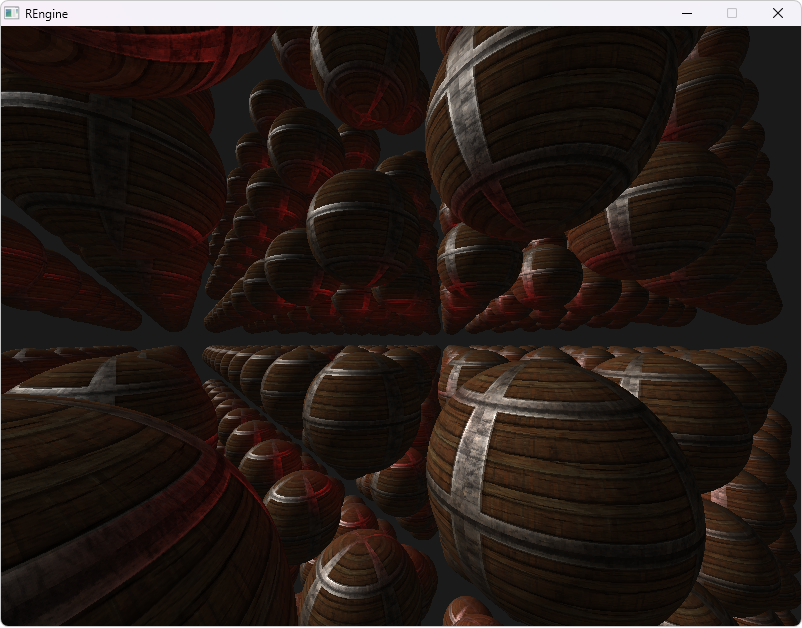
\includegraphics[width=1\linewidth]{culling.png}}
\caption{Сцена, тестирующая функционал отсечения невидимых поверхностей}
\label{culling:image}
\end{figure}
